%%%%%%%%%%%%%%%%%%%%%%%%%%%%%%%%%%%%%%%%%
% Fancyslides Presentation
% LaTeX Template
% Version 1.0 (30/6/13)
%
% This template has been downloaded from:
% http://www.LaTeXTemplates.com
%
% The Fancyslides class was created by:
% Paweł Łupkowski (pawel.lupkowski@gmail.com)
%
% License:
% CC BY-NC-SA 3.0 (http://creativecommons.org/licenses/by-nc-sa/3.0/)
%
%%%%%%%%%%%%%%%%%%%%%%%%%%%%%%%%%%%%%%%%%

%----------------------------------------------------------------------------------------
%	PACKAGES AND OTHER DOCUMENT CONFIGURATIONS
%----------------------------------------------------------------------------------------

\documentclass{fancyslides}

\usepackage[utf8]{inputenc} % Allows the usage of non-english characters
\usepackage{times} % Use the Times font
\usepackage{booktabs} % Allows the use of \toprule, \midrule and \bottomrule in tables
\graphicspath{{images/}} % Location of the slide background and figure files

% Beamer options - do not change
\usetheme{default} 
\setbeamertemplate{navigation symbols}{} % Disable the slide navigation buttons on the bottom of each slide
\setbeamercolor{structure}{fg=\yourowntexcol} % Define the color of titles and fixed text elements (e.g. bullet points)
\setbeamercolor{normal text}{fg=\yourowntexcol} % Define the color of text in the presentation

%------------------------------------------------
% COLORS
% The following colors are predefined in this class: white, black, gray, blue, green and orange

% Define your own color as follows:
%\definecolor{pink}{rgb}{156,0,151}

\newcommand{\structureopacity}{0.75} % Opacity (transparency) for the structure elements (boxes and circles)

\newcommand{\strcolor}{blue} % Set the color of structure elements (boxes and circles)
\newcommand{\yourowntexcol}{black} % Set the text color

%----------------------------------------------------------------------------------------
%	TITLE SLIDE
%----------------------------------------------------------------------------------------

\newcommand{\titlephrase}{Plasma Physics Term Project Presentation } % Presentation title
\newcommand{\name}{Anil Aksu} % Presenter's name
\newcommand{\affil}{Middle East Technical University} % Presenter's institution
\newcommand{\email}{aksu.anil@metu.edu.tr} % Presenter's email address

\begin{document}

\startingslide % This command inserts the title slide as the first slide

%----------------------------------------------------------------------------------------
%	PRESENTATION SLIDES
%----------------------------------------------------------------------------------------

\fbckg{re-entry.jpg} % Slide background image
\begin{frame}
\framedsl{Atmospheric Re-entry Problem} % Text in this environment is printed in a circle and will be made large and uppercase - if you need to fit more text in you can reduce the font size within the \pointedsl{} bracket as usual, e.g. \pointedsl{\large smaller main point}
\end{frame}

%------------------------------------------------

\fbckg{blank} % Slide background image
\begin{frame}
   \frametitle{Atmospheric Conditions}
The atmosphere consists of 6 layers which are Troposphere, Stratosphere, Mesosphere, Ionosphere, Thermosphere and Exosphere. 
  	  \begin{figure}
\label{fig:Atmosphere}
  \centering
      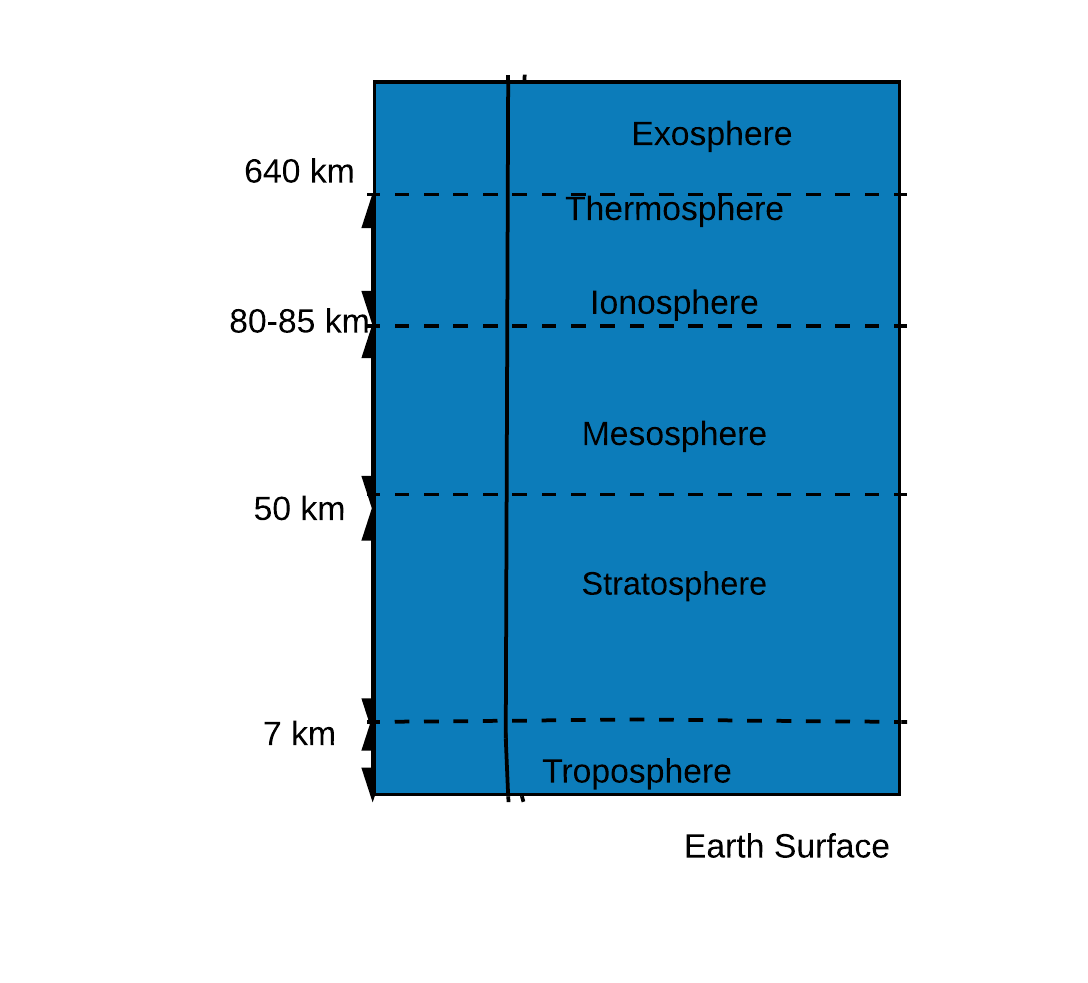
\includegraphics[scale=0.2]{AtmosphereLayers.png}
\end{figure}
 \end{frame}
 
 \fbckg{blank}
 \begin{frame}
   \frametitle{Atmospheric Conditions}
   \misc{ % Anything can be placed inside the \misc{} command
   \begin{itemize}
   \item \emph{ \color{yellow} Troposphere:} {\small The troposphere is the lowest part of the atmosphere and  also where almost all weather takes place.} 
   \\
   \item \emph{ \color{yellow} Stratosphere:} {\small The second region of atmosphere extending upward from the tropopause characterized by vertical gradient in temperature which triggers internal waves within Stratosphere. }
   \item \emph{ \color{yellow} Mesosphere:} {\small The mesosphere is directly above the stratosphere. Temperature decreases with height throughout the mesosphere with minimum $183K$.}
   \item \emph{ \color{yellow}Ionosphere:} {\small The layer of atmosphere that is ionized by solar and cosmic radiation with temperature cycles within $200K$-$500K$.}
   \item \emph{ \color{yellow} Thermosphere:}{\small The region of the atmosphere where a continuous medium assumption fails.}
   \item \emph{ \color{yellow} Exosphere:}{\small The uppermost layer, where the atmosphere diminishes and merges with interplanetary space.}
   \end{itemize}
}

\end{frame}

%------------------------------------------------

\fbckg{blank} % Slide background image
\begin{frame}

 \frametitle{Re-entry Problem}
 
   \begin{figure}
\label{fig:Rocket}
  \centering
      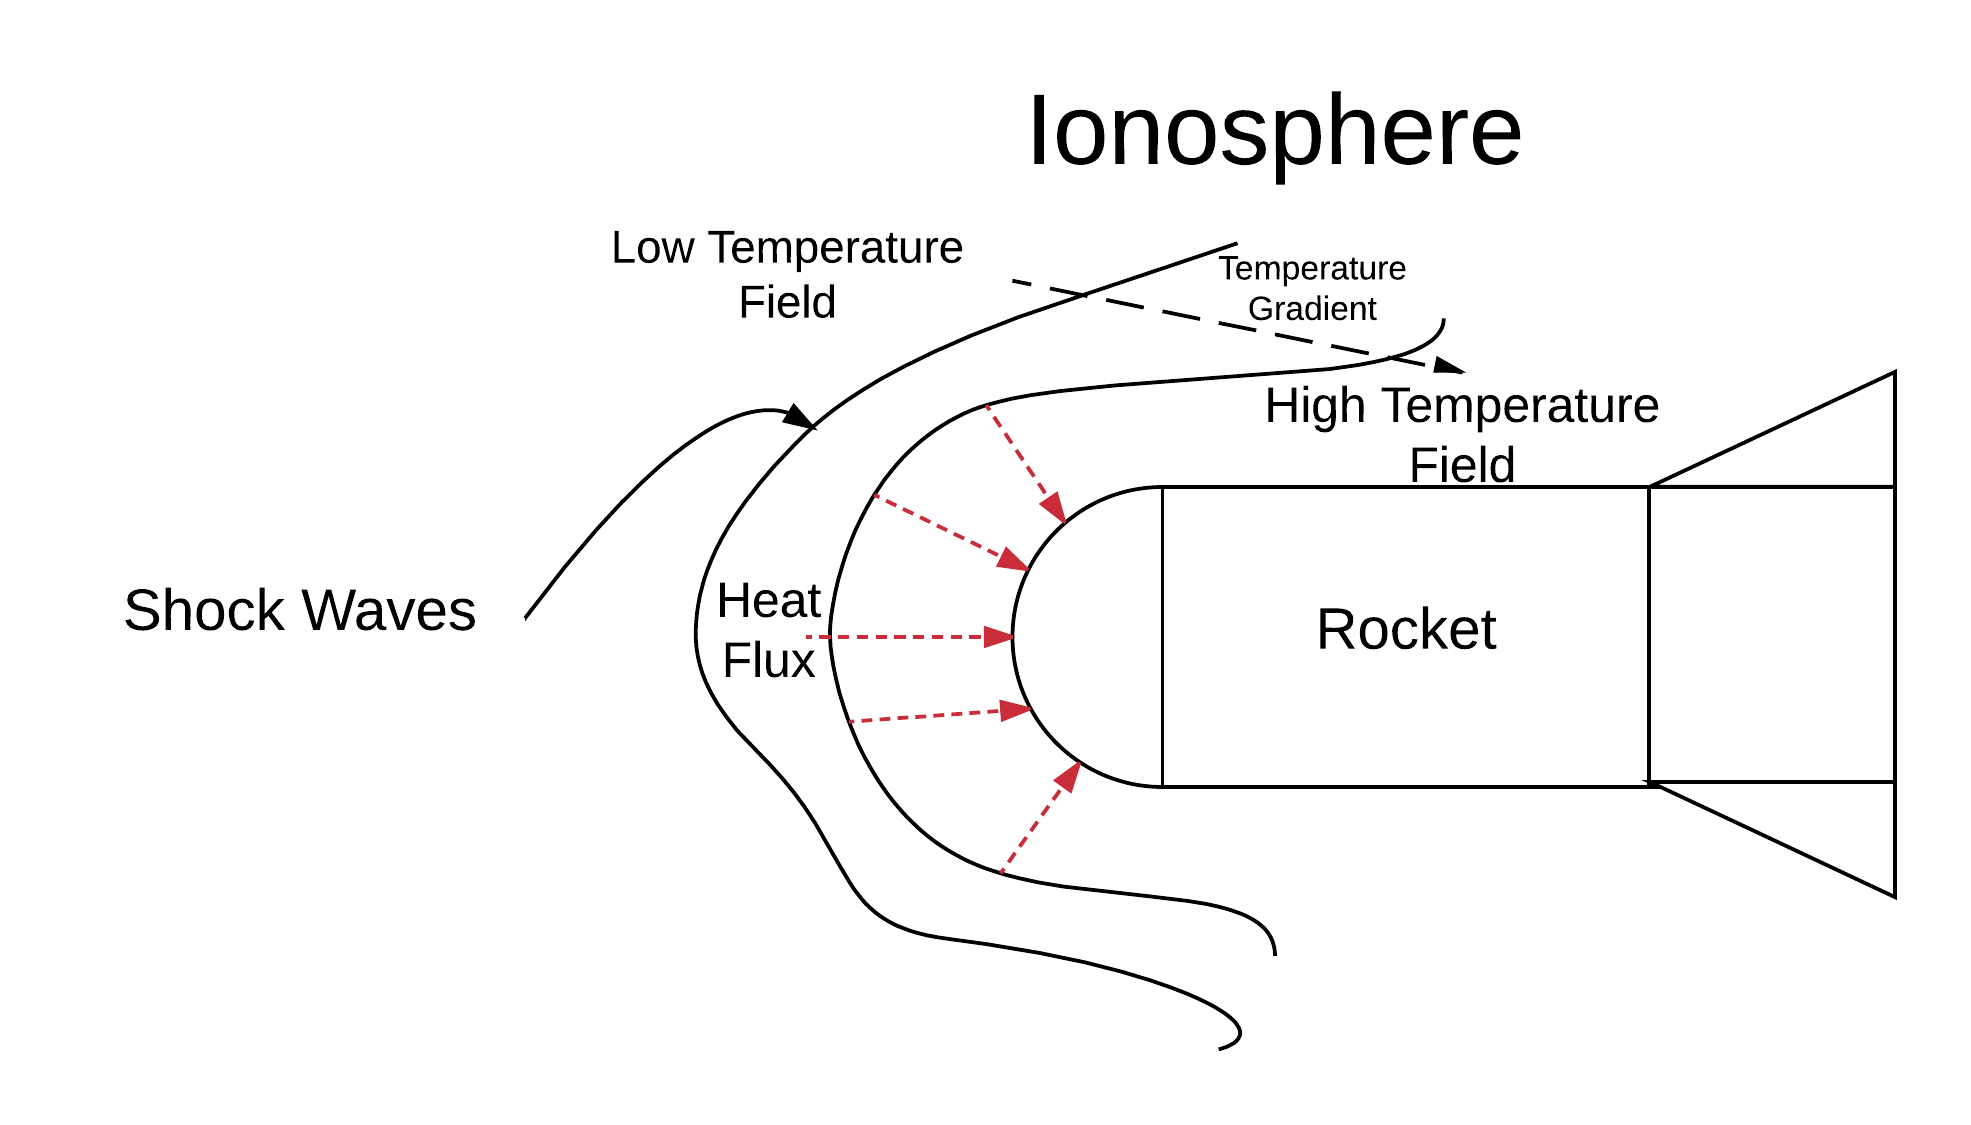
\includegraphics[scale=0.13]{Rocket.png}
\end{figure}
\begin{itemize}
\item \emph{ \color{purple} Abrupt changes in state quantities such as temperature and density.}
\item \emph{ \color{purple} Consequently, destructive thermo-mechanical effects on a rocket or a space vehicle \cite{Votta}.}
\item \emph{ \color{purple} Possible destructive electromagnetic effects \cite{Savino,Votta} as well.}
\end{itemize}

\end{frame}

%------------------------------------------------

\fbckg{blank} % Slide background image
\begin{frame}
 \frametitle{Objective}
\misc{ % Anything can be placed inside the \misc{} command
\begin{itemize}
   \item {\small \emph{ \color{yellow} Understanding the behaviour of shocks in Ionosphere:}}  How the magnetic field and the electric field induced by ions and electrons affect the shock surface.
   \item  {\small \emph{ \color{yellow} How the presence of shock affects the electric field and the magnetic field:}}If there exist and abrupt change in the electric and the magnetic fields before and after shock layer.
   \item  {\small \emph{ \color{yellow} How the geometric design and the material selection of a rocket can be modified to overcome the disruptive effects of a shock wave:}}There is a sudden increase in temperature field after shock surface around the rocket. These may be overcome by improving the design of the rocket.
   \end{itemize}
}
\end{frame}

\fbckg{blank} % Slide background image
 
\begin{frame}
\frametitle{Methods of Analysis}
\misc{ % Anything can be placed inside the \misc{} command
\begin{itemize}
   \item \emph{ \color{yellow} Single Fluid Magneto-Hydrodynamic Model:} {\small It is derived under continuum assumption by summing of momentum and energy equations of each species.} 
   \\
   \item \emph{ \color{yellow} Simplified 1-D Analytical Gas Dynamic Model:} {\small It is a basis for estimating and validating more advanced analysis tools. }
   \item \emph{ \color{yellow} 2-D Spectral Element MHD Numerical Model:} {\small It is a state of art numerical scheme used to produce more realistic results for the atmospheric re-entry problem.}

   \end{itemize}
}
\end{frame}
%------------------------------------------------

\fbckg{blank} % Slide background image

\begin{frame}
 \frametitle{Magneto-hydrodynamic Flows}
 the continuity is given as:
\begin{equation}
\label{eq:1}
m_i\left [\frac{\partial n_i}{\partial t}+\frac{\partial n_i u_j  }{\partial x_j}\right ]=0. 
\end{equation}
The momentum equations for each species are given as:
\begin{equation}
\label{eq:2}
 \sum_{i} m_i n_i \left [\frac{\partial \rho \mathbf{u}_i}{\partial t}+ u_{i}^{j}\frac{\partial \mathbf{u}_i}{\partial x_j}    \right ]=-\mathbf{\nabla}p_i+n_i q_i \mathbf{E}+\mu \nabla^2 \mathbf{u}_i+R_{ik}(\mathbf{u}_k-\mathbf{u}_i),
\end{equation}
The energy equation\cite{UCL} is given as:
\begin{equation}
\label{eq:3}
\sum_{i} m_i n_i c_{p_i} \left ( \frac{\partial T_i}{\partial t}+u_{i}^{j}\frac{\partial T_i}{\partial x_j}\right )=2\mu \mathbf{D}_{i}^{mn}\mathbf{D}_{i}^{mn}+\kappa \nabla^2 T_i.
\end{equation}
where  $c_{p_i}$ is heat capacitance and
\begin{equation}
\label{eq:4}
\mathbf{D}_{i}^{mn}=
\begin{bmatrix}
\frac{\partial u_{i}^{x}}{\partial x} & \frac{1}{2}(\frac{\partial u_{i}^{x}}{\partial y}+\frac{\partial u_{i}^{y}}{\partial x}) \\ 
\frac{1}{2}(\frac{\partial u_{i}^{x}}{\partial y}+\frac{\partial u_{i}^{y}}{\partial x}) & \frac{\partial u_{i}^{y}}{\partial y} 
\end{bmatrix}
\end{equation}
\end{frame}

%------------------------------------------------

\fbckg{blank} % Slide background image

\begin{frame}
 \frametitle{Magneto-hydrodynamic Flows: Continued}
 The electric field $\mathbf{E}$ can be formulated in terms of a potential field $\phi$.
\begin{equation}
	\mathbf{E}=-\mathbf{\nabla}\phi.
\end{equation}
and also 
\begin{equation}
	\epsilon_0 \mathbf{\nabla}^2 \phi=e(n_e-Zn_i).
\end{equation}
Finally, the pressure term can be found by utilizing the state equation:
\begin{equation}
p_i=n_i \gamma T_i
\end{equation}
\end{frame}
%------------------------------------------------



\fbckg{blank} % Slide background image
\begin{frame}
 \frametitle{Shocks In Compressible Flows: 1-D Model}
 The mass continuity:
\begin{equation}
\label{eq:220}
\frac{\partial \rho}{\partial t}+ \frac{\partial \rho u}{\partial x}=0,
\end{equation}
The momentum equation:
\begin{equation}
\label{eq:221}
\frac{\partial \rho u}{\partial t}+ \frac{\partial }{\partial x}\left ( \rho u^2 +p -\frac{4 \mu}{3}\frac{\partial u}{\partial x} \right )=0,
\end{equation}
The energy equation:
\begin{equation}
\label{eq:222}
\frac{\partial }{\partial t}\left ( \frac{1}{2}\rho u^2 + \rho e \right )+ \frac{\partial }{\partial x}\left ( \rho u(\frac{u^2}{2}+h)-\frac{4 \mu}{3}u\frac{\partial u}{\partial x}-\kappa \frac{\partial T}{\partial x} \right )=0.
\end{equation}

where $\mu$ is viscosity and $\kappa$ is conductivity.
\end{frame}

\fbckg{blank} % Slide background image
\begin{frame}
 \frametitle{Shocks Conditions In Compressible Flows}
\begin{columns}
\begin{column}{0.5\textwidth}
   \begin{center}
     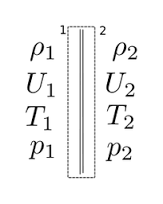
\includegraphics[width=0.5\textwidth]{shock.png}
     \end{center}
  by Green's theorem around infinitely thin shock surface: 
\begin{equation}
\label{eq:1}
	\oint_{C}f(\rho) \mathrm{d} t-\rho \mathrm{d} x =0.
\end{equation}
It results in:
\begin{equation}
	[\rho]\mathrm{d} x=[f(\rho)]\mathrm{d} t.
\end{equation}
\end{column}
\begin{column}{0.5\textwidth}  %%<--- here
the difference between the quantities $[f(\rho)]=f(\rho ^+)-f(\rho ^-)$ and $[\rho]=\rho ^+-\rho ^-$ are given in bracket notation.
    \begin{center}
     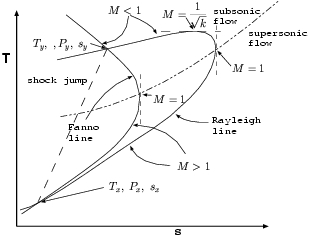
\includegraphics[width=1.\textwidth]{shockTS.jpg}
     \end{center}
\end{column}
\end{columns}

\end{frame}

%------------------------------------------------
\fbckg{blank} % Slide background image
\begin{frame}
 \frametitle{Numerical Method: Spectral Element Method}
Any quantity can be given as:
\begin{equation}
\label{eq:30}
u=\sum_{i=1}^{N_x}\sum_{j=1}^{N_y}\alpha_{ij}(t) P_i(x)P_{j}(y),
\end{equation}
Legendre polynomial are orthogonal set of functions on their mother interval $x\in[-1,1]$, therefore:
\begin{equation}
\label{eq:32}
<P_n(x)P_m(x)>\int_{-1}^{1}P_n(x)P_m(x)\mathrm{d}x=\frac{2}{2+n}\delta_{mn}.
\end{equation}
In case of weak formulation, the governing equations are multiplied with $P_i(x)P_j(y)$ and integrated over whole domain.
\end{frame}
%------------------------------------------------
\fbckg{blank} % Slide background image
\begin{frame}
 \frametitle{Numerical Method: Operator Splitting}
{ \Large \emph{ \color{blue} The time integration is performed in two steps:}}
\\
\emph{ \color{purple} First Step}: Integration of non-linear, electro-magnetic and pressure terms are performed explicitly,
 \begin{equation}
[\mathbf{M}]\frac{u^{*}-u^{n}}{\Delta t}=N_{term}^{n}+E_{term}^{n}+P_{term}^{n}
 \end{equation}
 where $[\mathbf{M}]$ is the mass matrix generated by weak formulation.
 \emph{ \color{purple} Second Step}: Integration of diffusive terms are performed implicitly,
 \begin{equation}
[\mathbf{M}]\frac{u^{n+1}-u^{*}}{\Delta t}=[\mathbf{K}]u^{n+1}
 \end{equation}
 where $[\mathbf{K}]$ is the matrix generated by weak formulation of diffusive terms.
 \\
\emph{ \color{purple} Notice}: Implicit formulation is preferred for the stability of the time integration.
\end{frame}


%------------------------------------------------
\fbckg{blank} % Slide background image
\begin{frame}
 \frametitle{Results: 1-D Analytical Shock Solution In Compressible Flows }
For large and small Prandtl number which is defined as $Pr=\mu Cp/\kappa$, the steady-state solution to the set of equations\cite{Johnson} above is given as:
\begin{equation}
\label{eq:223}
x=\frac{2 L_k}{\gamma+1}\log \left [(v_0 -v)^{v_0/(v_0-v_1)}(v-v_1)^{-v_1/(v_0-v_1)}  \right ].
\end{equation}
where $L_k= \kappa_0/m_0 Cv $.
\begin{columns}
\begin{column}{0.5\textwidth}
   \begin{center}
     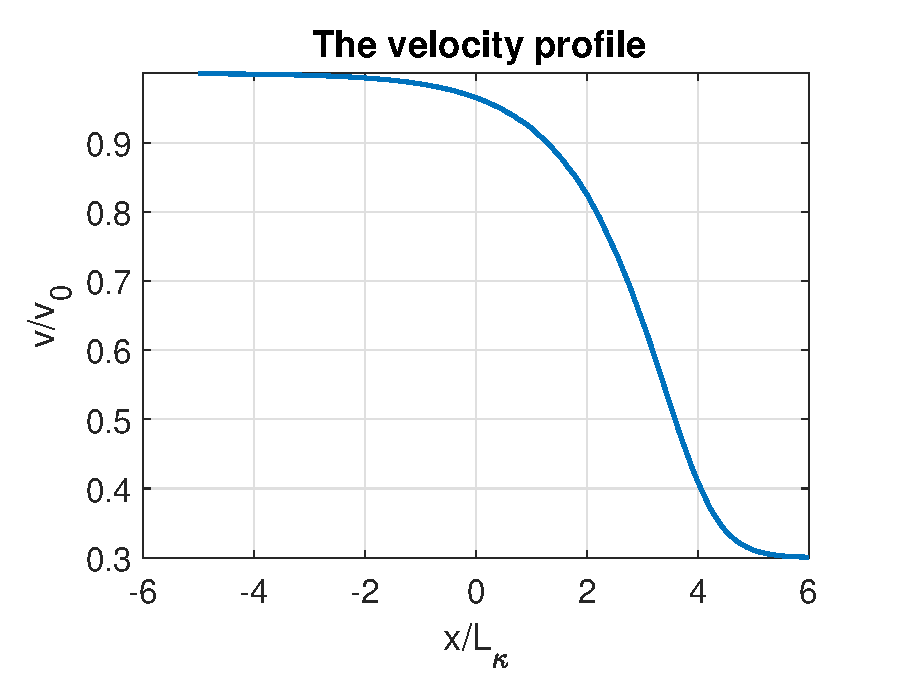
\includegraphics[width=1.\textwidth]{1DVel.eps}
     \end{center}

\end{column}
\begin{column}{0.5\textwidth}  %%<--- here
    \begin{center}
     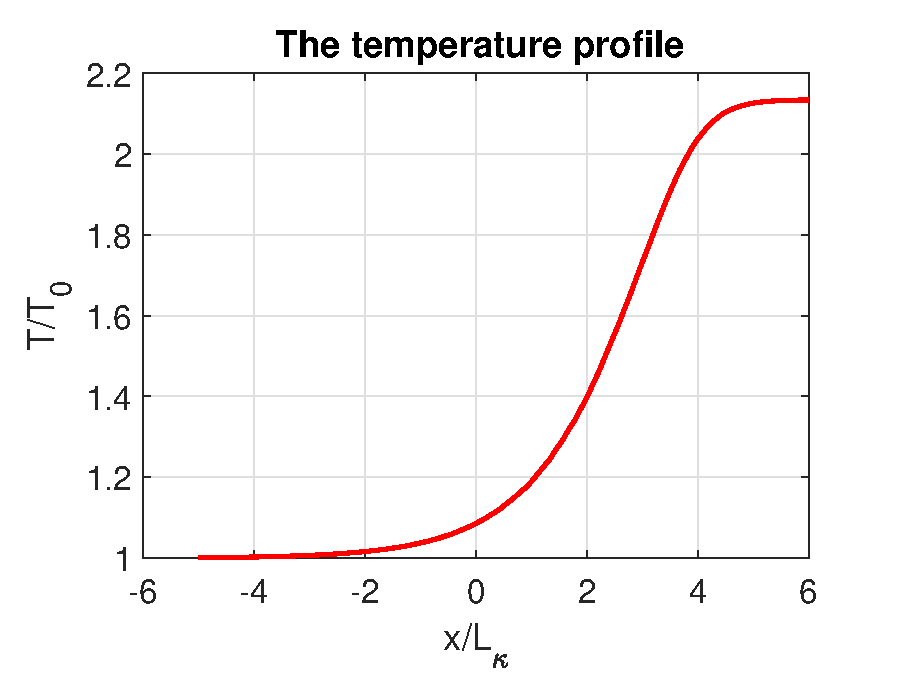
\includegraphics[width=1.\textwidth]{1DTemp.eps}
     \end{center}
\end{column}
\end{columns}
\end{frame}
%------------------------------------------------
\fbckg{blank} % Slide background image
\begin{frame}
 \frametitle{Results: 2-D Numerical MHD Solution}
 { \Large \emph{ \color{blue} Induced Electric Field in various time steps}}
\begin{columns}
\begin{column}{0.5\textwidth}
   \begin{center}
     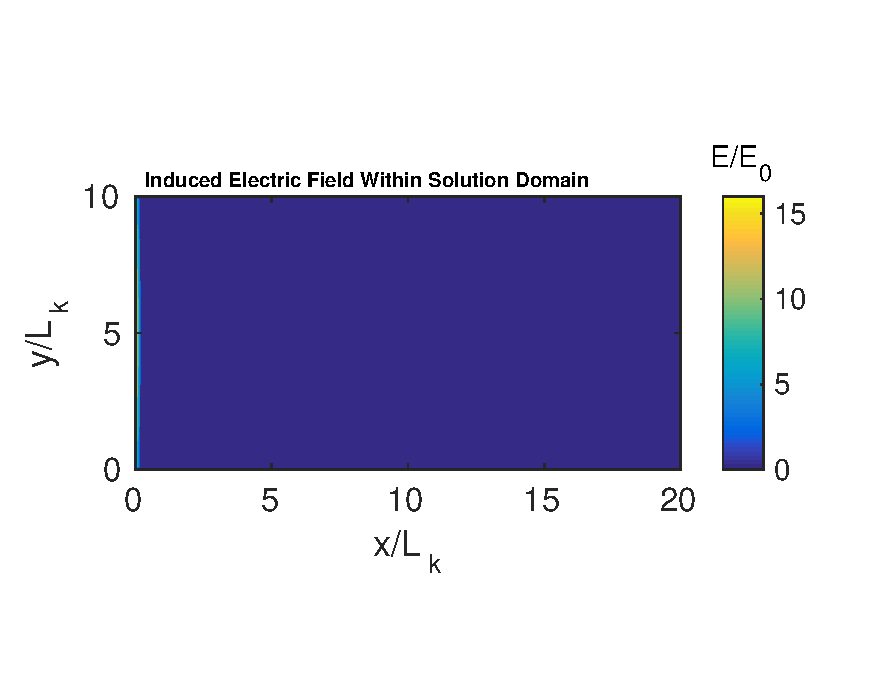
\includegraphics[width=0.9\textwidth]{Ebeg.eps}
     \end{center}
 \begin{center}
     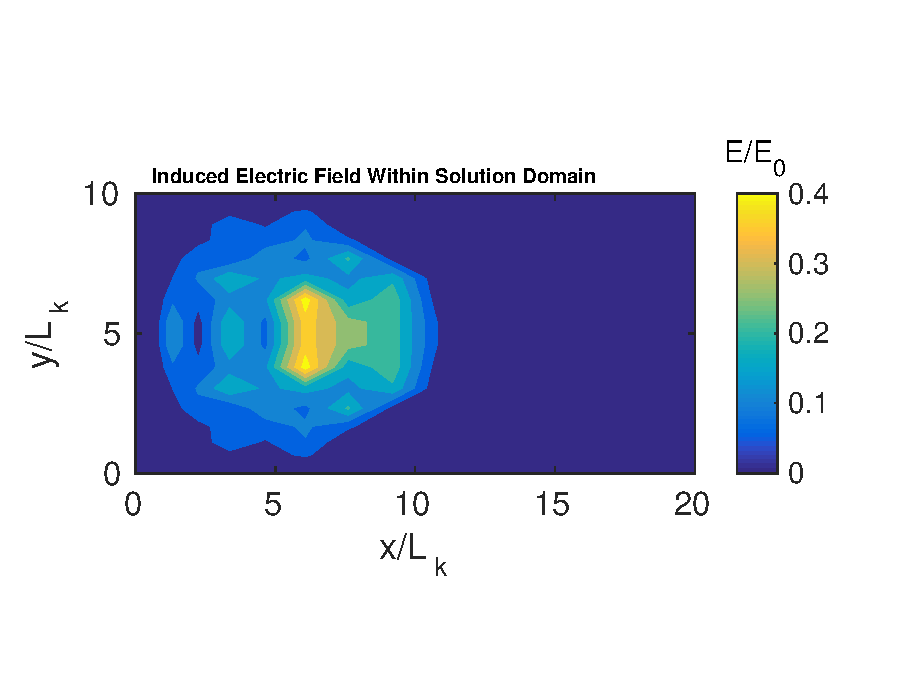
\includegraphics[width=0.9\textwidth]{Emid1.eps}
     \end{center}
\end{column}
\begin{column}{0.5\textwidth}  %%<--- here
\begin{center}
     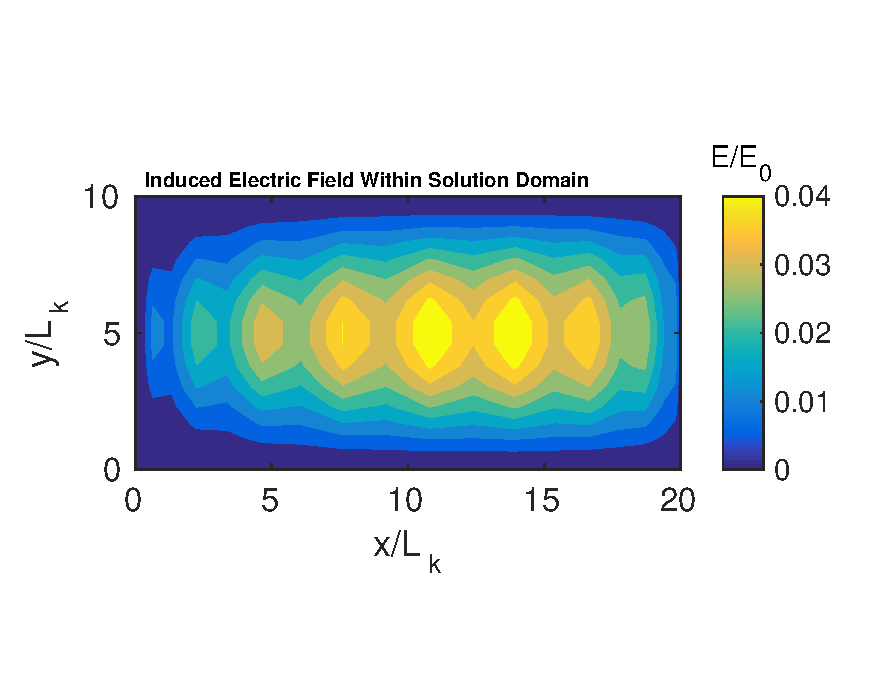
\includegraphics[width=0.9\textwidth]{Emid2.eps}
     \end{center}
    \begin{center}
     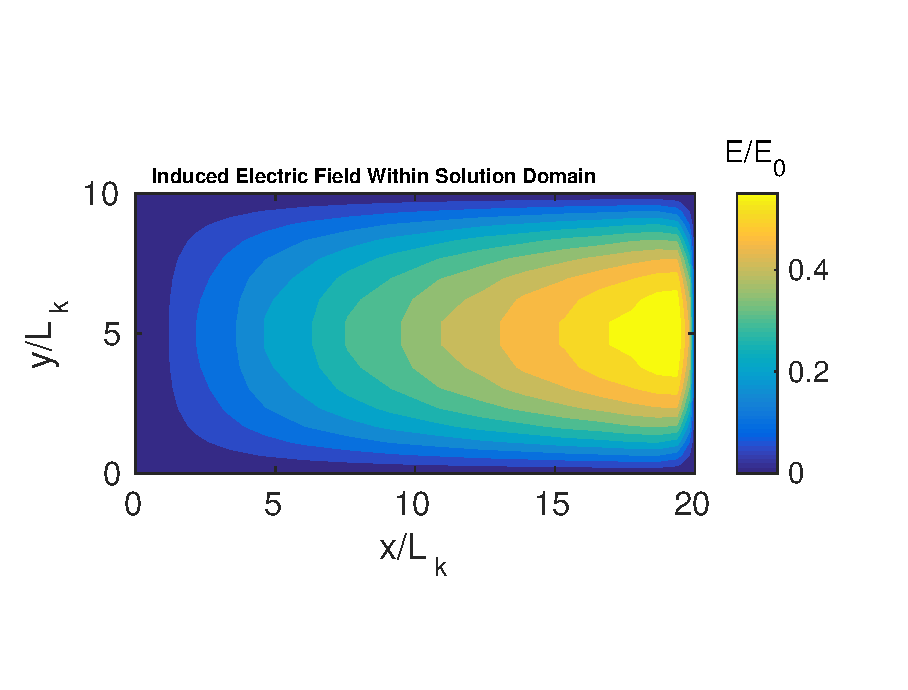
\includegraphics[width=0.9\textwidth]{EFinal.eps}
     \end{center}
\end{column}
\end{columns}
\end{frame}
%------------------------------------------------
\fbckg{blank} % Slide background image
\begin{frame}
 \frametitle{Conclusion}
\misc{ % Anything can be placed inside the \misc{} command
 \emph{ \color{yellow} The effects of compressibility is significant in the atmospheric re-entry problem:}
\begin{itemize}
 
   \item \emph{ \color{black} The presence of shock leads to a dramatic temperature increase around a re-entry vehicle or rocket.}  
   \\
   \item \emph{ \color{black} Since the charged particles accumulates in the region after shock, there is also a significant increase in electric field after shock layer. }
 
   \end{itemize}
   
   \emph{ \color{yellow} 2-D Spectral Element Method is an accurate numerical algorithm to analyze MHD problem with shock layers:}
\begin{itemize}
 
   \item \emph{ \color{black}It gives high resolution in space and time.}  
   \\
   \item \emph{ \color{black}A finer mesh around the shock layer enables to get more detailed description of flow conditions. }
 
   \end{itemize}   
    
}
\end{frame}
%------------------------------------------------
\fbckg{1.jpg} % Slide background image
\begin{frame}
 \frametitle{Future Work}
\misc{ % Anything can be placed inside the \misc{} command
\begin{itemize}
 
   \item \emph{ \color{yellow} Implementation of Statistical Model:} {\small Vlasov Equations describe the motion of plasma more accurately.} 
  \item \emph{ \color{yellow}  3-D Spectral Element MHD Numerical Model:} {\small The more realistic case would occur in 3-D model, possibly more complex dynamics would take place. }
   \item \emph{ \color{yellow} Extension to Non-rectangular Geometries:} {\small These methodologies are supposed to be applied to space vehicles or rockets, therefore it is supposed to be extrapolated to more realistic geometries.}

   \end{itemize}
}
\end{frame}
%------------------------------------------------
\fbckg{blank} % Slide background image
\begin{frame}
 \frametitle{References}
\bibliographystyle{plain}
\bibliography{mybib}% Produces the bibliography via BibTeX.
\end{frame}


\fbckg{kurtcobain.jpg} % Slide background image
\begin{frame}
\framedsl{Thank You} 
%\thankyou % Inserts a thank you slide
\end{frame}

%------------------------------------------------

%\fbckg{blank} % A blank background can be used instead of an image
%\begin{frame}
%\sources{ % An environment for giving credit for slide backgrounds, images will need to be scaled down if there are more than two
%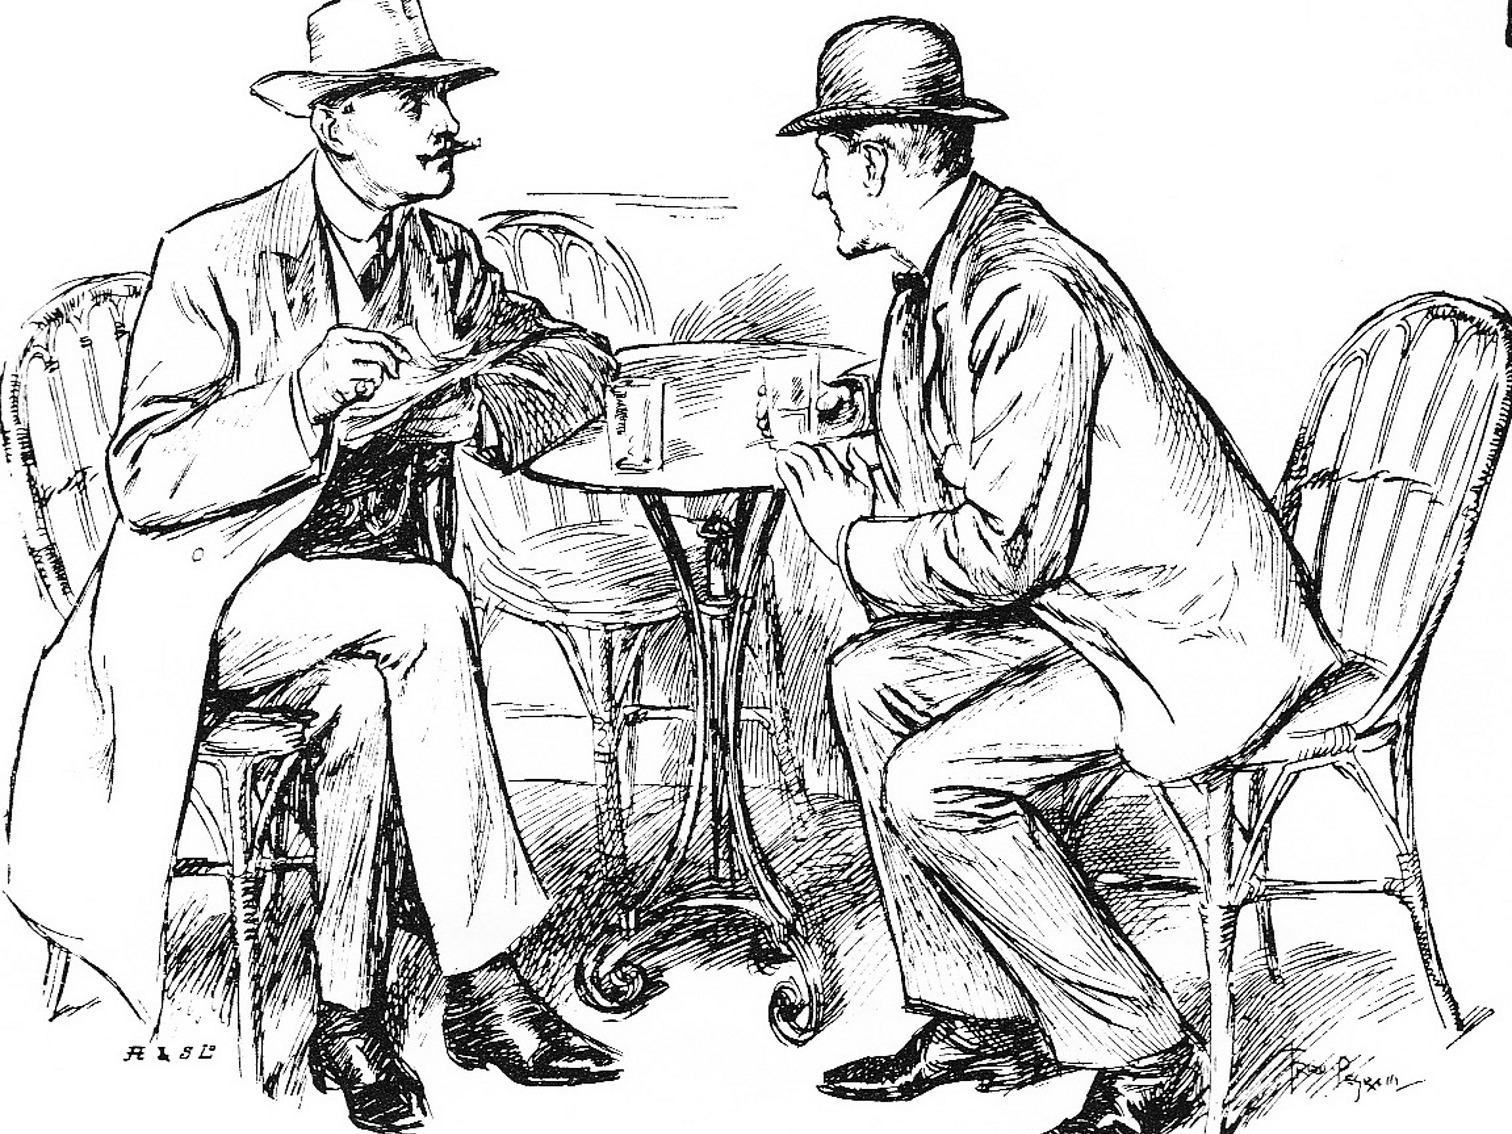
\includegraphics[scale=0.048]{1.jpg} \ flickr/lovelornpoets\\
%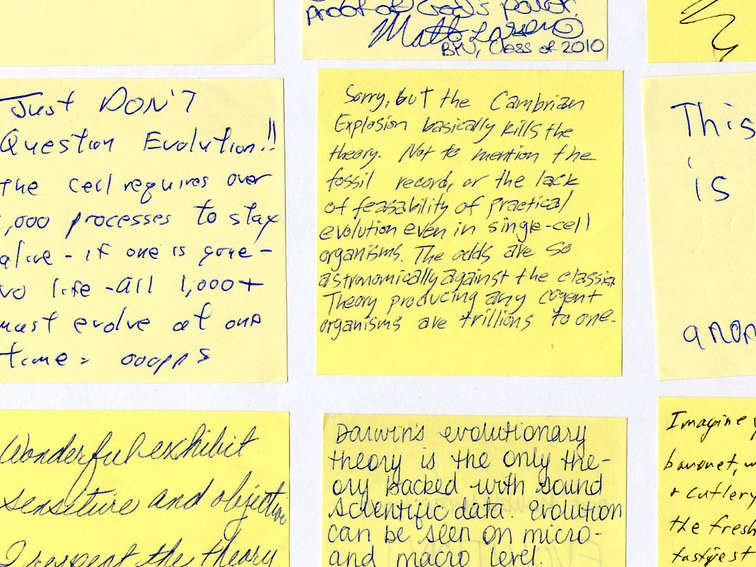
\includegraphics[scale=0.2]{2.jpg} \ flickr/apsmuseum
%}
%\end{frame}

%----------------------------------------------------------------------------------------

\end{document}